\documentclass[12pt,a4paper]{report}
\usepackage{graphicx}
\usepackage{amsmath}
\usepackage{fancyhdr}
\usepackage{cite}
\usepackage{framed}
\usepackage{a4wide}
\usepackage{float}
\graphicspath{ {./frontpages/} }
%The below Section make chapter and its name to center of the page
\usepackage{blindtext}
\usepackage{xpatch}
\makeatletter
\xpatchcmd{\@makeschapterhead}{%
  \Huge \bfseries  #1\par\nobreak%
}{%
  \Huge \bfseries\centering #1\par\nobreak%
}{\typeout{Patched makeschapterhead}}{\typeout{patching of @makeschapterhead failed}}


\xpatchcmd{\@makechapterhead}{%
  \huge\bfseries \@chapapp\space \thechapter
}{%
  \huge\bfseries\centering \@chapapp\space \thechapter
}{\typeout{Patched @makechapterhead}}{\typeout{Patching of @makechapterhead failed}}

\makeatother
%The above Section make chapter and its name to center of the page
%\unwanted packages also included

\linespread{1.5}
%\pagestyle{fancy}
%\fancyhead{}
%\header and footer section
%\renewcommand\headrulewidth{0.1pt}
%\fancyhead[L]{\footnotesize \leftmark}
%\fancyhead[R]{\footnotesize \thepage}
%\renewcommand\headrulewidth{0pt}
%\fancyfoot[R]{\small College of Engineering, Kidangoor}
%\renewcommand\footrulewidth{0.1pt}
%\fancyfoot[C]{2019 - 2020}
%\fancyfoot[L]{\small Name of the project}




\begin{document}
\begin{center}
{\Large \textbf{TRANSISTORS BASED ON TWO-DIMENSIONAL MATERIALS
FOR FUTURE INTEGRATED CIRCUITS
}}\\
\vspace{2cm}
A SEMINAR REPORT\\
\vspace{0.5cm}
Submitted by \\
\vspace{1cm}
<<<<<<< HEAD
\textbf{safhkjdgdgk}\\
=======
\textbf{ADARSH S}\\
>>>>>>> 5d1d1f1f97a77b234b641a8b10220ad3f6d429fd
\vspace{0.2cm}
\textbf{KGR18EC002}\\
\vspace{0.2cm} to\\


 the A P J Abdul Kalam Technological University \\
in partial fulfillment of the requirements for the award 
of the Degree \\
of\\
Bachelor of Technology \\
in\\
Electronics and Communication Engineering
\end{center}


\begin{center}

\vspace{1.2cm}


\includegraphics[scale=0.3]{ceklogo.jpg}

DEPARTMENT OF ELECTRONICS \& COMMUNICATION ENGINEERING\\

COLLEGE OF ENGINEERING KIDANGOOR\\

JANUARY 2022\\
\end{center}

\thispagestyle{empty}
\newpage
%\Declaration in this page.
\begin{center}
\textbf{DECLARATION}\\
\end{center}
I hereby declare that the seminar report \textbf{“Transistors based on Two-Dimensional Materials
for Future Integrated Circuits”}, 
submitted for partial fulfillment of the requirements for the award of degree of 
Bachelor of Technology in Electronics and Communication Engineering of the APJ 
Abdul Kalam Technological University, Kerala is a bonafide work done by me
under supervision of Mr. Joby James, Assistant Professor of Electronics and Communication Engineering Department. 
This submission represents my ideas in
 my own words and where ideas or words of others have been included, I 
 have adequately and accurately cited and referenced the original sources. 
 I also declare that I have adhered to ethics of academic honesty and 
 integrity and have not misrepresented or fabricated any data or idea 
 or fact or source in my submission. I understand that any violation 
 of the above will be a cause for disciplinary action by the Institute 
 and/or the University and can also evoke penal action from the sources 
 which have thus not been properly cited or from whom proper permission 
 has not been obtained. This report has not been previously formed the 
 basis for the award of any degree, diploma or similar title of any other 
 University.

\noindent \begin{minipage}{0.45\linewidth}
\begin{flushleft}
\vspace{1 cm}
                         
Kidangoor \\
17/01/2022\\

\end{flushleft} 
\end{minipage}
\hfill
\begin{minipage}{0.45\linewidth}
\begin{flushright}                                      
\vspace{1cm}
                         
ADARSH S\\


\end{flushright} 
\end{minipage}

\thispagestyle{empty}

\newpage
\begin{center}

%\vspace{1.5cm}

\textbf{Department of Electronics and Communication Engineering}

\textbf{COLLEGE OF ENGINEERING KIDANGOOR}


\textbf{2018-2022}
\end{center}
\begin{center}

\includegraphics[scale=0.25]{ceklogo.jpg}

\end{center}
\vspace{0.2cm}
\begin{center}
 \textbf{CERTIFICATE}
\end{center}
% him/her => 
This is to certify that the report entitled \textbf{ \large TRANSISTORS BASED ON TWO-DIMENSIONAL MATERIALS
FOR FUTURE INTEGRATED CIRCUITS} 
submitted by \textbf{ADARSH S}, to the APJ Abdul Kalam Technological University in 
partial fulfillment of the Bachelor of Technology degree in Electronics 
and Communication Engineering is a bonafide record of the seminar work 
carried out by him under our guidance and supervision.
\vspace{3cm}

\noindent \begin{minipage}{0.45\linewidth}
\begin{flushleft}
\vspace{3cm}
                         
\textbf{Seminar Coordinator} \\
\vspace{0.8cm}
Joby James \\
\footnotesize{Assistant Professor\\
Electronics and Communication\\
College of Engineering Kidangoor}\\

\end{flushleft} 
\end{minipage}
\hfill
\begin{minipage}{0.35\linewidth}
\begin{flushleft}                                      
\vspace{3cm}
                         
\textbf{Head of the Department} \\
\vspace{.8cm}
Syama R\\
\footnotesize{Assistant Professor\\
Electronics and Communication\\
College of Engineering Kidangoor}\\


\end{flushleft} 
\end{minipage}
\thispagestyle{empty}

\newpage
\chapter*{\centering \large ACKNOWLEDGEMENT\markboth{Acknowledgements}{Acknowledgements}}

This is the most satisfying, yet most difficult part of the 
seminar to present gratifying
words because most often they fail to convey the real 
influence, others have had on one’s
work.First and foremost I thank The Almighty for his 
abundant blessings without which
this seminar would not have been success. I am extremely 
grateful to Dr. K G Viswanadhan, Principal, College of 
Engineering Kidangoor, for providing with best facilities. 
I would
like to extend my sincere gratitude to Ms. Syama R,
Assistant Professor and Head of the
Department of Electronics and Communication Engineering for 
extending every facility to
complete my seminar work successfully.I would like to 
express my sincere indebtedness to
Asst. Professor Joby James of Department of Electronics 
and Communication Engineering, for his valuable guidance,
wholehearted co-operation and duly approving the topic as
staff in charge. I also thank all my teachers and friends 
for their sincere guidance and cooperation. Above all I 
thank my parents who have been the pillars of support 
and constant encouragement throughout the course of this seminar



\begin{flushright}
\textbf{ADARSH S}
\end{flushright}
\thispagestyle{empty}


% Please remove and edit percentage(%) Symbol, if you want this 
% Acknowledgement page in your report. As per ktu guideline, 
% this page is not necessary. 
\begin{abstract}

%\pagenumbering{roman}
Field-effect transistors based on two-dimensional (2D) materials have the potential to be used in very large-scale integration (VLSI) technology, but whether they can be used at the front end of line or at the back end of line through monolithic or heterogeneous integration remains to be determined. To achieve this, multiple challenges must be overcome, including reducing the contact resistance, developing stable and controllable doping schemes, advancing mobility engineering and improving high-κ dielectric integration. The large-area growth of uniform 2D layers is also required to ensure low defect density, low device-to-device variation and clean interfaces. Two-dimensional (2D) materials hold great promise for future nanoelectronics as conventional semiconductor technologies face serious limitations in performance and power dissipation for future technology nodes. The atomic thinness of 2D materials enables highly scaled field-effect transistors (FETs) with reduced short-channel effects while maintaining high carrier mobility, essential for high-performance, low-voltage device operations. The richness of their electronic band structure opens up the possibility of using these materials in novel electronic and optoelectronic devices. These applications are strongly dependent on the electrical properties of 2D materials-based FETs. Thus, accurate characterization of important properties such as conductivity, carrier density, mobility, contact resistance, interface trap density, etc is vital for progress in the field. 


\end{abstract}
\pagenumbering{roman}
\tableofcontents %This command used for index.
\listoffigures




    

\chapter{INTRODUCTION}
\pagenumbering{arabic}
The scaling of silicon complementary metal–oxide– semiconductor (CMOS) technology has reached sub-10-nm technology nodes, but further scaling is increasingly challenging because the gate electrostatics of the devices demand an aggressive reduction in channel thickness to preserve the desired performance. The ultimate channel thickness for a field-effect transistor (FET) is potentially in the sub-1-nm range. However, this is not readily accessible for any three-dimensional (3D) semiconducting crystal because of increased scattering of charge carriers at the channel-to-dielectric interfaces, which leads to severe mobility degradation. Two-dimensional (2D) semiconducting materials, which in monolayer form have a thickness of ~0.6 nm, could provide a solution. Such materials include transition metal dichalcogenides (TMDs) with the general formula MX2, where M is a transition metal (for example, Mo or W) and X is a chalcogen (for example, S, Se or Te). The absence of dangling bonds in the materials also offers the potential to achieve better channel-to-dielectric interfaces. Early studies based on mechanically exfoliated single-crystalline 2D flakes, and more recent developments based on large-area grown synthetic 2D monolayers, have illustrated the promising characteristics of 2D transistors. However, the multitude of challenges that remain to be solved makes the potential incorporation of 2D FETs in future very large-scale integration (VLSI) technologies far from clear. 

Two-dimensional (2D) van der Waals materials or layered materials are characterized by materials with an anisotropic electronic and chemical structure of strong covalent bonds along the in-plane direction and weak van der Waals bonds along the out-of plane direction. Among such materials, graphene has been studied most extensively, due to its high mobility, widely tunable carrier concentration, and the occurrence of phenomena such as the quantum Hall effect in atomically thin samples prepared by a simple Scotch tape exfoliation method. Subsequently, the development of large-scale chemical vapor deposition (CVD) graphene synthesis has enabled the fabrication of wafer-scale electronic and photonic devices.  Meanwhile, theoretical studies on carrier transport in graphene have inspired experimental research in the fields of condensed matter physics, semiconductor nanoelectronics, photonics, and energy storage. In addition to graphene, other 2D materials have been investigated with great intensity for future electronic and optoelectronic applications, as these materials offer a range of bandgaps with high carrier mobility and efficient electrostatic control. These properties, combined with mechanical flexibility and tunability of electronic properties, make 2D materials especially promising as a channel material in high-performance 2D field effect transistors (FETs), which could be operated in emerging future mobile and IoT environment. In light of this, accurate characterization of 2D FETs and extraction of important device parameters, such as resistivity, carrier density, mobility, contact resistance, charge trap densities, dielectric permittivity, and anisotropy in carrier transport, are essential to explore 2D materials and to correlate them with the performance of 2D FETs. 

It is critically important to understand the electrical properties of such devices, since the use of conventional electrical characterization methods can produce unreliable results when applied to ultra-thin 2D layered materials. For example, room-temperature electrical conductivity in a bulk semiconductor is directly related to charge carrier density. However, conventional implanted substitutional doping cannot be performed on 2D materials due to their atomic thinness. Instead, different methods, such as charge transfer doping, are predominantly used to generate electron and hole carriers in 2D materials, and in few-layer materials, the charge density falls off rapidly away from the surface, rather than being uniform as in conventional semiconductor materials. Furthermore, the pristine surface of 2D materials forms weak van der Waals bonds with adjacent materials and presents challenges to the creation of low-resistance contacts, by introducing a tunnel barrier for charge carrier transport, whereas the formation of stronger bonds requires disruption of the 2D crystal structure, which introduces defect states. Therefore, it is important to accurately characterize the properties of metal contacts, e.g., contact resistance and metal-semiconductor Schottky barrier. Interfaces between 2D semiconductors and metals are subject to Fermi level pinning due to the tunnel barrier at the interface, defect-induced interface states, and orbital overlap between adjacent heterogeneous materials, requiring precise characterization of the Schottky barrier and Fermi level pinning, which could severely increase the contact resistance at the interfaces .



\section{Moore's Law}
Moore's law is the observation that the number of transistors in a dense integrated circuit (IC) doubles about every two years. Moore's law is an observation and projection of a historical trend. Rather than a law of physics, it is an empirical relationship linked to gains from experience in production. The observation is named after Gordon Moore, the co-founder of Fairchild Semiconductor and Intel (and former CEO of the latter), who in 1965 posited a doubling every year in the number of components per integrated circuit, and projected this rate of growth would continue for at least another decade. 

Moore's prediction has been used in the semiconductor industry to guide long-term planning and to set targets for research and development, thus functioning to some extent as a self-fulfilling prophecy. Advancements in digital electronics, such as the reduction in quality-adjusted microprocessor prices, the increase in memory capacity (RAM and flash), the improvement of sensors, and even the number and size of pixels in digital cameras, are strongly linked to Moore's law. 

In recent years, Moore’s Law has slowly fallen out of relevance. The predictions Moore made were related to the speed of innovation and that speed has slowed. The development of transistors based two dimensional material will enable Moore’s Law trend in the future. 



\begin{figure}
  \centering
  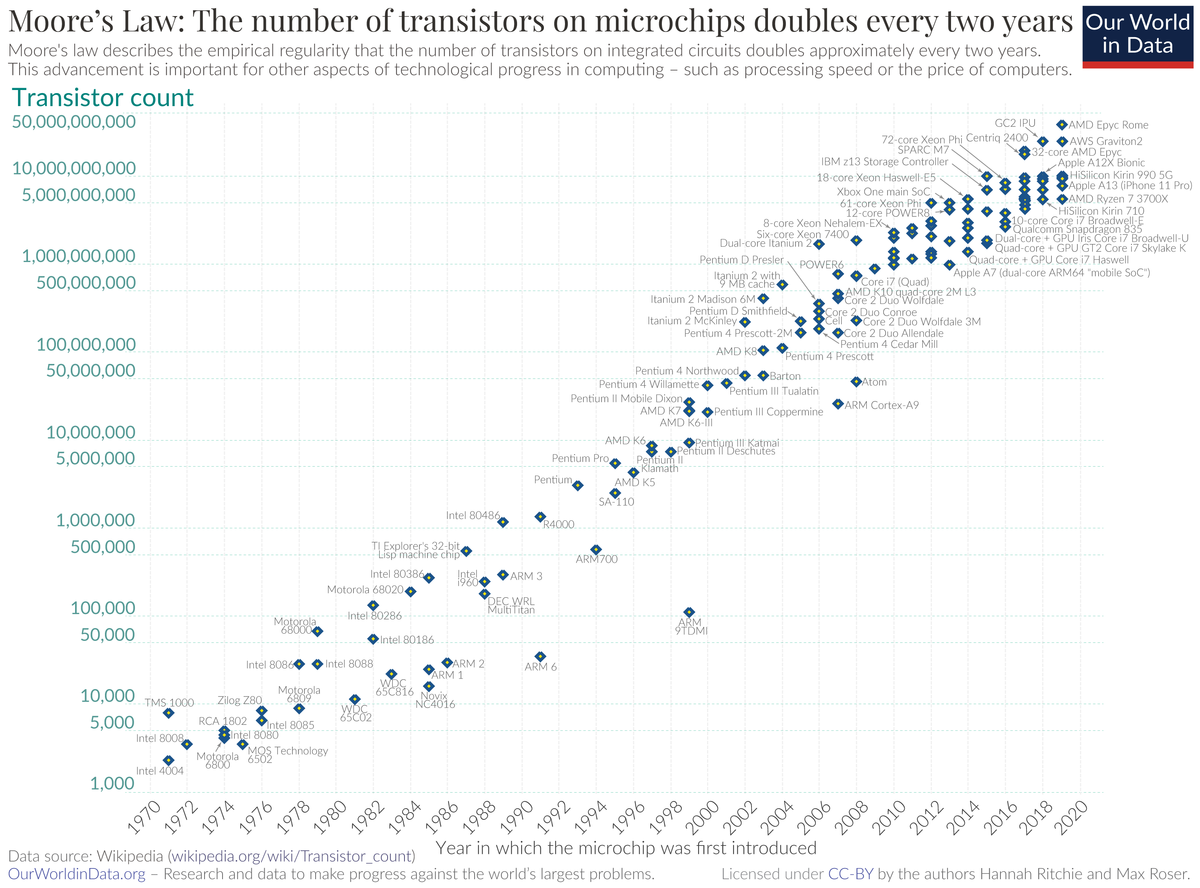
\includegraphics[scale=0.3]{Moore's_Law_Transistor_Count.png}
  \caption{ A semi-log plot of transistor counts for microprocessors against dates of introduction, nearly doubling every two years.}
  \label{moores}
  \end{figure}

\chapter{Two-Dimensional Materials}
\section{Definition}

Two-dimensional (2D) materials are defined as crystalline materials consisting 
of single- or few-layer atoms, in which the in-plane interatomic interactions 
are much stronger than those along the stacking direction. Since the success of 
monolayer graphene exfoliation, 2D materials have been extensively studied due
 to their unique structures and unprecedented properties. 

\section{Introduction}
Two-dimensional (2D) materials are defined as crystalline materials consisting of single- or few-layer atoms, in which the in-plane interatomic interactions are much stronger than those along the stacking direction. Since the first exfoliation of single-layer graphene, 2D materials have attracted worldwide attention due to their unique structures and remarkable properties. For example, graphene composed of hexagonally arranged sp2 hybridized atoms possesses extraordinary strength, giant carrier mobility, extremely high thermal conductivity, and excellent optical properties compared to the existing materials. These exceptional properties and single-atomic-layer structures enable graphene to have a wide range of applications in field-effect transistors, flexible electronics, photodetectors, composite materials, energy storage, precise sensors, DNA sequencing and drug delivery.

The rapid and prosperous development of graphene stimulates numerous research interests on other 2D materials. More than one thousand structures of 2D materials have been predicted to be easily exfoliated to monolayers or multilayers with fascinating physical properties, forming a large family of 2D materials. The booming synthetic methods established from graphene have brought experimental realizations of dozens of novel 2D crystals. Monolayer MoS2 and hexagonal boron nitride (h-BN) have been extracted at an early stage and have recently received much attention. Some graphene analogs such as black phosphorene, borophene, silicene, germanane, stanene, antimonene, bismuthene and tellurene have been synthesized in the past few years. Although these 2D materials have an atomic layer structure similar to that of graphene, their physical properties are distinct from those of graphene. Thus, these 2D materials can act as complementary materials and have the potential for broader applications. For example, unlike graphene, phosphorene has a strong in-plane structural anisotropy, leading to a significant dependence of the material properties on its orientation. For electronic properties, graphene has a direct zero band gap and exhibits a certain metallicity. Other 2D crystals have a large variety of band structures. The direct band gaps of h-BN, MoS2, and WSe2 allow them to be promising materials for optical devices, transistors, phototransistors, and photodetectors. The metallic electronic character possessed by borophene and VS2 is essential for electronic and energy storage applications. In addition, stanene, as a 2D topological insulator, is theoretically predicted to display superconductivity at the edges. A large number of 2D material family members could satisfy variant requirements for a huge diversity of applications. The structure and mechanics of 2D materials play important roles in manufacturing, integration, and performance for their potential applications.

During the synthesis of 2D materials, various types of defects are inevitably generated. For example, during the chemical vapor deposition (CVD) process for the large-area growth of graphene, many isolated grains from different nucleation sites stitch into uniform structures, leading to the formation of grain boundaries (GBs) between neighbouring grains with a misorientation . Furthermore, graphene’s irradiation or chemical treatment can generate various point defects, such as dislocations, vacancies, and functionalized groups. The majority of experimental studies have shown that these defects in 2D crystals significantly affect their physical, chemical, and mechanical properties. In particular, it has been demonstrated that defects can tailor the properties of 2D materials via the controlled arrangement of defects. Therefore, the concepts of defect engineering and topological design have emerged and been used to achieve tunable properties of 2D materials.



\section{Classification and Atomic Structures}

The 2D material family has extended to more than one thousand members based on theoretical predictions. To date, tens of these materials have been synthesized experimentally. Generally, 2D materials can be categorized into four types (including graphene family, Xenes, chalcogenides, and 2D oxides) according to their components and atomic structures.

The graphene family contains graphene and its derivatives consisting of different hybridized carbon atoms or heterogeneous element. In fluoro-graphene, chloro-graphene, and graphene oxide, the saturated carbon atoms (sp3 hybridization) bind with noncarbon elements, forming an alternating pattern. Carbon allotropes (such as graphyne) are constructed by the network of sp- and sp2-hybridized carbon atoms. The graphyne structure can be regarded as replacing partial aromatic C–C bonds in graphene with acetylene chains. Complete, 2/3, 1/3 and 5/12 replacements result in α-, β-, γ- and 6,6,12-graphyne, respectively. Graphyne structures exhibit fascinating semiconducting properties, enabling their use in electronic devices. These structures are also thought to be possible candidates in gas separation, filtration, and water desalination because of their intrinsic nanopores. Analogous to graphene, two or more elements can substitute the original carbon atoms to form more complex layered systems, such as h-BN , boron–carbon–nitrogen (BCN), and SixC1−x . In addition to the analogous hexagonal structure above, a 2D material with a tetragonal arrangement is also predicted to be considerably stable. The p(pi)–d(pi) bonded TiC is buckled into a zigzag line in the side view. Such a distinguished structure endows it with anisotropic properties.

\begin{figure}
  \centering
  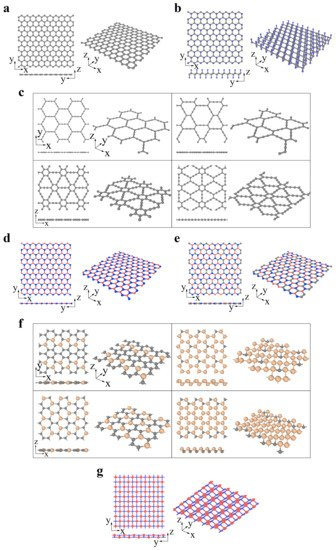
\includegraphics[scale=0.3]{2.1.jpg}
  \caption{The graphene family: (a) graphene (gray atom represents C), (b) CX (X = H, F, Cl; gray and blue atoms represent C and X, respectively), (c) graphyne (α-graphyne, β-graphyne, γ-graphyne and 6,6,12-graphyne from left to right, top to bottom; gray atom represents C), (d) h-BN (red and blue atoms represent B and N, respectively), (e) BCN (reproduced from Ref.; red, gray and blue atoms represent B, C and N, respectively), (f) SixC1−x(x = 2/10, 5/6, 2/6, 14/18 from left to right, top to bottom; gray and yellow atoms represent C and Si, respectively) (reproduced from Ref.), (g) TiC (reproduced from Ref.; red and blue atoms represent C and Ti, respectively).}
  \label{graphenefam}
  \end{figure}

<<<<<<< HEAD
  The solid red line shows the locus of points for which the
DOF is 0.5 mm; in the region to the left of that line the
DOF values are larger. Points in the region between the
two lines correspond to situations in which the resolution
is 100 nm or better, and the DOF is 0.5 mm or longer. As
shown, to be in this favorable region, the wavelength of
the light used for imaging must be less than 40 nm, and
the NA of the imaging system must be less than 0.2. The
solid circle shows the parameters used in current imaging
experiments. Light having wavelengths in the spectral
region from 40 nm to 1 nm is variously referred to as
extreme uv, vacuum uv, or soft x-ray radiation.
Projection lithography carried out with light in this
region has come to be known as EUV lithography
(EUVL). Early in the development of EUVL, the
technology was called soft x-ray projection lithography
(SXPL), but that name was dropped in order to avoid
confusion with x-ray lithographyy, which is a 1:1, 
near contact printing technology


As explained above, EUVL is capable of printing features
of 100 nm and smaller while achieving a DOF of 0.5 mm
and larger. Currently, most EUVL work is carried out in
a wavelength region around 13 nm using cameras that
have an NA of about 0.1, which places the technology
well within the “Comfort Zone for Manufacture” as
shown in Figure 1 by the data point farthest to the right.

% Lithography with 193 nanometer light has been 
% pushed further than many would 
% have thought possible, but it has come at a cost: 
% the industry has had to reach 
% deep into a bag of tricks to continue shrinking 
% chip features. Chipmakers will be 
% able to continue making smaller, faster and 
% more powerful chips while keeping 
% costs in check.


% \begin{figure}
% \centering
% \includegraphics[scale=0.5]{Substrate.jpg}
% \caption{Elements of Biological cells and components of a typical IoT device.}{Ref- [2]}
% \label{sub}
% \end{figure}

\section{Working}

EUVL is a significant departure from the deep 
ultraviolet lithography standard. 
Attached to the EUV scanner, the source consists 
of a droplet generator, collector and a vacuum chamber. 
In EUV, the process takes place in a vacuum 
environment, because nearly everything absorbs 
EUV light.(All optical elements, including the photomask,
 must use defect-free molybdenum/silicon (Mo/Si) 
 multilayers (consisting of 40 Mo/Si bilayers) that 
act to reflect light by means of interlayer 
interference; any one of these mirrors absorb
 around 30\% 
of the incident light). The source of the light is a tiny little droplet of tin.
they're smaller than 
the diameter of a human hair in which it fire 
across the vessel and then it is intercepted those 
with a pulsed laser 
beam of very high power and have to hit with 
an accuracy of just a few microns
The droplets are 25 microns in diameter and 
are falling at a rate of 50,000 times a second
In the vessel, there is a camera. A droplet 
passes a certain position in the chamber. 
Then, the camera tells the seed laser in the 
sub-fab to fire a laser pulse into the main 
vacuum chamber. This is called the pre-pulse
The pre-pulse laser hits the spherical tin droplet 
and turns it into a pancake-like shape. Then the laser 
unit fires again, representing the main pulse. 
The main pulse hits the pancake-like tin droplet
 and vaporizes it.


At that point, the tin vapor becomes plasma. 
The plasma, in turn, emits EUV light at 13.5nm 
wavelengths. The goal is to hit a droplet with precision
This determines how much of the laser power 
gets turned into EUV light, 
which is referred to as conversion efficiency
There's a collector mirror that collects that light
and sends it into the scanner. then there are 
four mirrors that essentially shape that light 
into a slit that bounces off the reticle.
The light bounces off the collector and travels 
through an intermediate focus unit into the scanner
and what's happening next is step and scan. which 
basically means it continues to reproduce that 
particular pattern over and over again
EUV light is propelled into the scanner. In the 
scanner, the light bounces off a complex scheme 
of 10 surfaces or multi-layer mirrors. First, 
the light goes through a programmable illuminator. 
This forms a pupil shape to illuminate the right 
amount of light for the EUV mask.
Then, EUV light hits the mask, which is also 
reflective. It bounces off six multi-layer 
mirrors in the projection optics. Finally, 
the light hits the wafer at an angle of 6\%.

% Photomask ?
\section{EUVL Photomasks}
EUVL masks are reflective, not transmissive, which is 
achieved by using multiple alternating layers of 
molybdenum and silicon. They consist of a patterned absorber of EUV radiation placed
on top of an ML reflector deposited on a robust and solid
substrate, such as a silicon wafer. Membrane masks are
not required. The reflectance spectrum of the mask must
be matched to that of the ML-coated mirrors in the
camera. It is anticipated that EUVL masks will be
fabricated using processing techniques that are standard
in semiconductor production. Because a 4:1 reduction is
used in the imaging, the size and placement accuracy of
the features on the mask are achieved relatively easily.

This is in contrast to conventional photomasks 
which work by blocking light using a single 
chromium layer on a quartz substrate. An EUV mask 
consists of 40 alternating silicon and molybdenum 
layers; this multilayer acts to reflect the extreme 
ultraviolet light through Bragg diffraction; 
the reflectance is a strong function of incident 
angle and wavelength, with longer wavelengths 
reflecting more near normal incidence and shorter 
wavelengths reflecting more away from normal incidence. 
The pattern is defined in a tantalum-based 
absorbing layer over the multilayer.
 The multilayer 
may be protected by a thin ruthenium layer.


Current EUVL systems contain at least two 
condenser multilayer mirrors, six projection multilayer 
mirrors and a multilayer object (mask). Since 
the mirrors absorb 96\% of the EUV light, the ideal 
EUV source needs to be much brighter than its 
predecessors. EUV source development has focused on 
plasmas generated by laser or discharge pulses. 
The mirror responsible for collecting the light is 
directly exposed to the plasma and is vulnerable 
to damage from high-energy ions and other 
debris[19] such as tin droplets, which require 
the costly collector mirror to be replaced every year.

Very precise  extremely flat micro-mirrors to 
focus the light onto the silicon wafer to 
produce even finer feature widths.



% \begin{figure}[ht]
% \centering
% \includegraphics[scale=0.5]{molec commun.jpg}
% \caption{Examples of Molecular Communication} {Ref- [2]}
% \label{commun}
% \end{figure}


\section{EUVL Photoresists}

Photoresists are a critical part of lithography. Resists are 
light-sensitive materials. 
They form patterns on a surface when exposed to light. For EUV, 
they are critical.
The basic requirements for EUVL resist are sensitivity, 
resolution, Line Width Roughness 
(LWR) or Line Edge Roughness (LER), outgassing, a pattern 
cross-sectional aspect ratio 
and profile, etch resistance, defect density, and 
reproducibility. Among them, 
it is a critical challenge to meet the requirements 
simultaneously on resolution, 
LWR, and sensitivity (RLS). EUVL uses Chemically Amplified 
Resist (CAR) due to 
the advantages of high sensitivity and resolution, but its 
LWR is relatively high, 
which becomes a significant issue. For the 22 nm feature, 
LWR should be 
controlled below 2 nm, which is about half of the current 
best available values
\section{Multilayer Reflectors}

In order to achieve reasonable reflectivities, the reflecting
surfaces in EUVL imaging systems are coated with
multilayer thin films (ML’s). These coatings consist of a
large number of alternating layers of materials having
dissimilar EUV optical constants, and they provide a
resonant reflectivity when the period of the layers is
approximately $\lambda/2$. Without such reflectors, EUVL
would not be possible. On the other hand, the resonant
behavior of ML’s complicates the design, analysis, and
fabrication of EUV cameras. The most developed and
best understood EUV multilayers are made of alternating
layers of Mo and Si, and they function best for
wavelengths of about 13 nm. Figure 3 shows the
reflectivity and phase change upon reflection for an
Mo:Si ML that has been optimized for peak reflectivity at
13.4 nm at normal incidence; similar resonance behavior
is seen as a function of angle of incidence for a fixed
wavelength. While the curve shown is theoretical, peak
reflectivites of 68\% can now be routinely attained for
Mo:Si ML’s deposited by magnetron sputtering

\chapter{ADVANATGES}


\begin{itemize}
  \item \textbf{High performance processors and memory: }The smaller 
  lithography means that you can pack more transistors into the 
  same amount of space. The more transistors you can pack into 
  the same space means you can make a more powerful processor. 
  That smaller lithography also means you can pack more 
  cores into the same space as well

  \item \textbf{Reduces the Number of masks: }EUVL enables the use 
  of only one mask exposure instead of multiexposure, EUV will 
  enable a number of critical layers to be printed in single 
  pattern, thus reducing both the number of process steps and 
  the critical masks.
  \item \textbf{Better performance and scalability: }Laser-produced 
  plasma sources have been shown to be the leading technology with 
  scalability to meet the requirements of ASML scanners and 
  provide a path toward higher power needed by lithography tools 
  as they evolve over their life cycle
  
  \item \textbf{Better pattern fidelity which allows higher flexibility : }Since extreme-ultraviolet lithography (EUVL) uses a much shorter wavelength than optical lithography, it should provide better pattern fidelity
=======
>>>>>>> b6ceabdcc27dc887127133ac626b22b8f4a8ce71

  Xenes are monoelement 2D materials organized into distorted hexagonal or trigonal lattices. The 2D Xenes can be made up of group IIIA, IVA, and VA elements, termed borophene, silicene, germanene, stanene, phosphorene, and antimonene when X = B, Si, Ge, Sn, P, and Sb, respectively Unlike the ideally flat structure of graphene, 2D Xenes prefer alternating out-of-plane atomic arrangements, resulting in an anisotropic lattice structure. Due to abundant components and unique structures, 2D Xenes exhibit excellent physical, chemical, and mechanical properties, enabling them to be promising agents for biosensors, bioimaging, therapeutic delivery, and theranostics.
  \begin{figure}
    \centering
    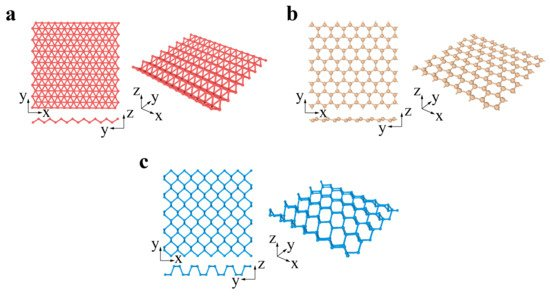
\includegraphics[scale=0.3]{2.2.jpg}
    \caption{Xenes: (a) borophene, (b) silicene, germanene, stanene and antimonene, (c) phosphorene.}
    \label{xenefam}
    \end{figure}
  
    Chalcogenides are a type of emerging 2D material represented by the transitional metal dichalcogenide (TMDC) MX2. For MX2, the layer of transitional metal atom M (Mo, W, Nb, Ta) is sandwiched by two layers of chalcogen atoms X (S, Se, Te). MX2 usually has two typical phases: 2H and 1T phases The 2H phases have been widely studied to date. The MX2 (M = Mo, W, Nb, Ta; X = S, Se, Te) prefers to be the 2H phase in equilibrium, while the MX2 (M = Zr, Hf; X = S, Se) prefers to be the 1T phase. The transformation from 2H to 1T phases can occur under specific conditions. GaS, GaSe, and InSe are chalcogenides with a double layer of metal intercalated between two layers of chalcogen, forming an X-M-M-X vertical structure. Bi2Te3, Bi2Se3, and Sb2Te3 belong to a specific branch of chalcogenides and are called topological insulators. There exists a van der Waals interaction between the stoichiometric monolayers, e.g., quintuple layers (QLs). A Bi2Se3 QL comprises five atomic layers stacked in the sequence of Se (1)-Bi-Se (2)-Bi-Se (1) along the c-axis.
    
    \begin{figure}
      \centering
      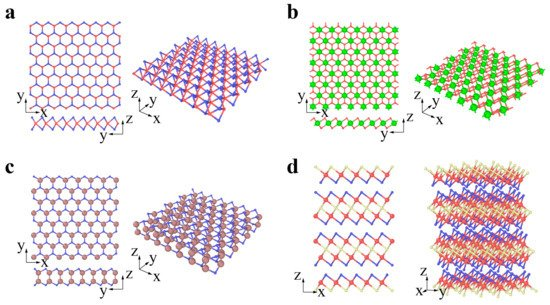
\includegraphics[scale=0.3]{2.3.jpg}
      \caption{Chalcogenides: (a) 2H-MX2 (M = Mo, W, Nb, Ta; X = S, Se, Te; red and blue atoms represent M and X, respectively), (b) 1T-MX2 (M = Zr, Hf; X = S, Se; green and red atoms represent M and X, respectively), (c) GaS, GaSe and InSe (brown and blue atoms represent Ga or In and S or Se, respectively), (d) Bi2Se3, Bi2Te3 and Sb2Te3 (red atoms represents Bi or Sb, while blue and yellow atoms represent Se or Te in different layers, respectively).}
      \label{xenefam}
      \end{figure}

      The common types of 2D oxides include lead, phosphorus, and transition metal oxides. 2D oxides usually appear as single planar structures and multilayer and superlattice structures. Layered 2D oxides have strong lateral chemical bonding in planes but exhibit weak van der Waals interactions between layers, while nonlayered 2D oxides (with superlattice structures) have atomic bonding in three dimensions. Many 2D oxides are functional materials with great potential in catalysis, energy storage, and electronics, since they have a highly chemically active interface.
      
      \begin{figure}
        \centering
        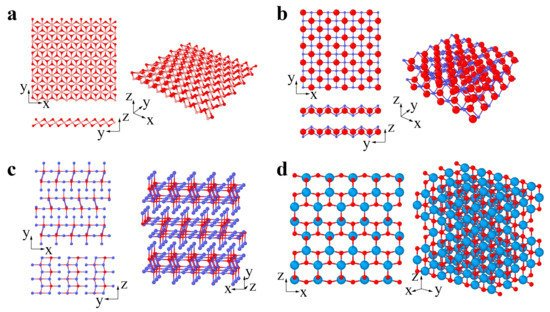
\includegraphics[scale=0.3]{2.4.jpg}
        \caption{2D oxides: (a) MnO2 (pink and red atoms represent Mn and O, respectively), (b) PbO (blue and red atoms represent Pb and O, respectively), (c) MoO3 (red and blue atoms represent Mo and O, respectively), (d) TiO2 (azure and red atoms represent Ti and O, respectively).}
        \label{xotherfam}
        \end{figure}

\section{Manufacturing of 2D Materials}
It is possible to take any material and thin it down (until it has a thickness of only a few atoms) to create a 2D material. However, many materials (e.g. diamonds) have chemical bonds oriented in 3-dimensions, so thinning the material requires cutting these bonds – leaving them ‘dangling’. A 2D material created in this way will have a high density of dangling bonds, which are chemically and energetically unstable, and can force the material to rearrange its structure to lower its surface energy.
Another allotrope of carbon – graphite – has strong chemical bonds only along planes within the bulk material. These planes are stacked on top of each other and held together by weak van der Waals interaction, and so can be separated without leaving any dangling bonds. In the case of graphite, a single plane is called graphene. Most of the 2D materials being studied therefore belong to the broader class of layered materials (or van der Waals materials).

There are two methods for making 2D materials:
i) Top-down (start with a bulk material and make it thinner) 
ii) Bottom-up (start with the atomic ingredients and assemble them together)
Within each of these approaches are several subcategories, each with their own advantages and disadvantages - explained below.

\subsection{Top-Down}

\subsubsection{Mechanical exfoliation}
Commonly known as the ‘Scotch-tape method’, it was first used to create monolayer graphene. A piece of sticky tape is applied to the surface of a layered material and then peeled off, taking flakes (consisting of a small number of layers) with it. The tape can then be pressed onto a substrate to transfer the flakes for study. The monolayer yield of this process is low (the flakes obtained are mostly multilayer), with no control over the size and shape. However, the size of monolayer flakes that can be produced is reasonable (from a few microns up to ~100 microns) and the quality of monolayers is excellent - with very few defects due to the lack of chemical processing involved.
It is also a suitable technique for all van der Waals materials. For these reasons, mechanical exfoliation remains popular for lab-based studies, but it is not scalable for integration into new technologies.

\begin{figure}
  \centering
  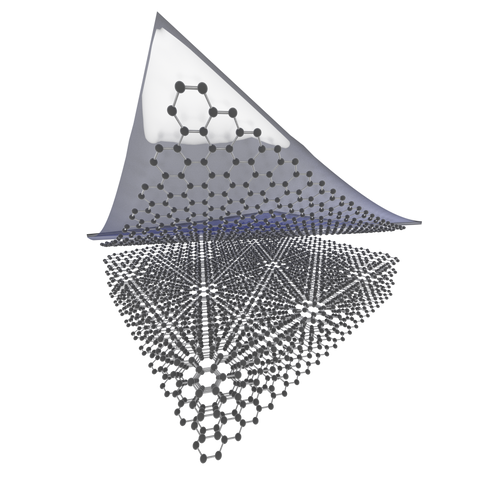
\includegraphics[scale=0.3]{2.1.1.png}
  \caption{Mechanical exfoliation involves peeling successive layers from a Van der Waals material using a tape}
  \label{mechexfol}
  \end{figure}

\subsubsection{Liquid exfoliation}
Another mechanical method, liquid exfoliation involves using an organic solvent as a medium to transfer mechanical force to the layered material (often in the form of a powder) suspended in the liquid. Sonication causes tensile stress to be applied to the layers, forcing them apart. To improve monolayer yield, variations exist - such as introducing reactive ions (between the material layers that create hydrogen bubbles) that push the layers apart, or that rapidly mix the solution to create additional shear force on the layers.
This method is highly scalable but has several drawbacks. The monolayer yield is again generally low, and the flakes are often less than 100 nm in size (due to the applied forces breaking them apart). The resultant flakes may also potentially have a high density of defects and residual solvent when removed from solution, making them unsuitable for many optoelectronic applications.
\begin{figure}
  \centering
  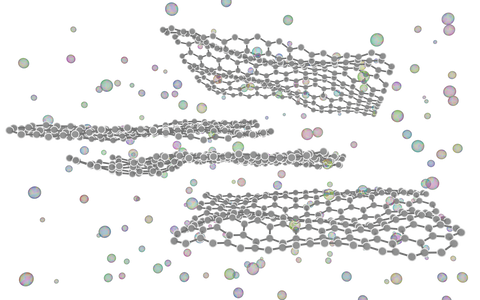
\includegraphics[scale=0.3]{2.1.2.png}
  \caption{Liquid exfoliation often uses bubbles to force layers apart.}
  \label{liqexfol}
  \end{figure}

\subsubsection{Chemical vapour deposition}
This process involves passing one or more precursor gases (which usually contain the atomic ingredients of the required film) through a heated furnace, where they will react together or with a substrate and form a thin layer of the required material. This process has been successfully applied to grow graphene and TMDCs. Several parameters (such as gas pressures and compositions, temperature, and reaction times) need to be controlled as they will affect the thickness, quality and composition of the films. While this process is more complex and expensive than most top-down techniques, it is highly scalable, and the quality of the films produced approaches that of mechanically-exfoliated layers.

\subsubsection{Solution-based chemical synthesis}
A vast variety of techniques have been developed to synthesise 2D materials through wet chemical techniques. These include high-temperature chemical reactions in solution, interface-mediated growth (reactions occur only at the surface of a liquid), fusion of nanoparticles into larger nanosheets, and many more. Each method is particularly well-suited to a certain type of 2D material, and everything from graphene and TMDCs to monolayer metals can be synthesised using the appropriate technique.
The lateral size of the flakes produced by these methods is generally small (<100’s nm), and the techniques share the same residual solvent problem as liquid exfoliation. However, for certain applications, the scalability, low cost and versatility of these techniques makes chemical synthesis the best method for large-scale production.
 


\section{Why are 2D materials different from bulk materials?}

This comes down to three reasons:
\subsubsection{Removal of van der Waals interactions }
A layered bulk material consists of many covalently-bonded planes held together by weak van der Waals interactions. When a force is applied to a material, these van der Waals forces can be easily overcome and the material breaks – making it seem weak. Conversely, the covalent bonds that hold the atoms together in the layers are actually very strong. A monolayer will only have covalent bonds. By removing the ‘weak links’ from the material, it appears to become much stronger. For example, graphene has a tensile strength 1000 times greater than graphite, and while a graphite pencil can be easily broken, graphene is over 100 times stronger than steel.
\subsubsection{An increase in the ratio of surface area-to-volume }
The surface area-to-volume ratio of a material defines how much of it is exposed to its environment. This is important for chemical reactions – the more reactant that is in contact with the material, the faster the reaction can occur, so 2D materials tend to be more reactive their bulk counterparts. It also makes 2D materials more sensitive to their surroundings, an effect that is exploited for sensors based on 2D materials.
\subsubsection{Confinement of electrons in a plane  }
The electronic and optical properties of a material depend upon its electronic band structure. This describes how electrons move through the material, and is a result of the periodicity of its crystal structure. When a material goes from bulk to 2D, the periodicity is removed in the direction perpendicular to the plane, which can greatly change the band structure. The modified band structures are responsible for the extremely high conductivity of graphene and the fluorescence of monolayer MoS2.
Another effect of dimensional confinement is reduced dielectric screening between electrons and holes in semiconductors. When there is less material to screen the electric field, there will be an increase in Coulomb interaction and more strongly-bound excitons – making them more stable than excitons found in bulk materials. If the excitons are confined in a plane that is thinner than their Bohr radius (as is the case for many 2D semiconductors), quantum confinement will result in an increase in their energy compared to bulk excitons, changing the wavelength of light they absorb and emit.
Their energy can be tuned somewhat by changing the number of layers in the 2D material (i.e. a bilayer structure will absorb/emit lower energy light than a monolayer). However, this can also affect the band structure, resulting in changes to other properties as well (for example, bilayer MoS2 becomes non-emissive compared to a monolayer due to changes in electronic band structure).
\begin{figure}
  \centering
  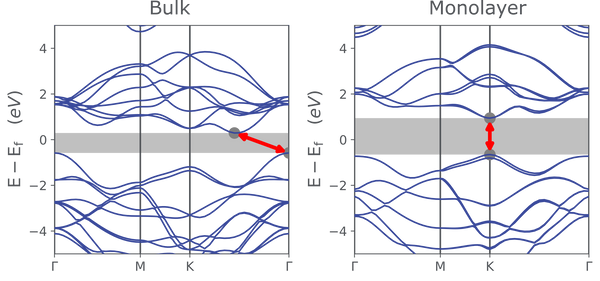
\includegraphics[scale=2]{2.2.1.png}
  \caption{Band structure diagram of (left) bulk and (right) monolayer MoS2 showing the crossover from indirect to direct bandgap accompanied by a widening of the bandgap.}
  \label{bandgap}
  \end{figure}

\chapter{TWO-DIMENSIONAL FET}
\section{Fundamentals of 2D material processing}
\begin{figure}
  \centering
  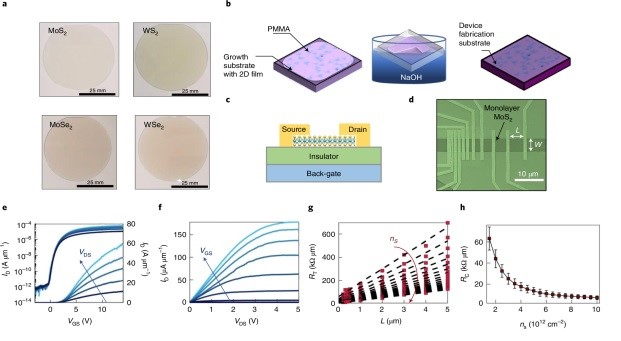
\includegraphics[scale=1]{twodimensionalfet.jpg}
  \caption{Two-dimensional FET fabrication and characterization. a, Epitaxial large-area growth of highly crystalline 2D monolayers on a sapphire substrate using a MOCVD technique by the Two-Dimensional Crystal Consortium (2DCC), an initiative of the National Science Foundation (NSF) through the Materials Innovation Platform (MIP). b, The poly(methyl methacrylate) (PMMA)-based wet-transfer technique developed by Zhang and others. c, Schematic of a 2D FET with global back-gate. d, SEM image of a TLM structure fabricated on monolayer MoS2. The channel is etched in a rectangular geometry to ensure constant channel width W. e,f, Transfer characteristics (that is, source-to-drain current, ID) measured by sweeping the gate voltage (VGS) at constant drain voltage (VDS), plotted in linear and logarithmic scale (e) and output characteristics obtained by measuring ID by sweeping VDS at
  constant VGS (f) of a 2D FET based on MOCVD-grown monolayer MoS2. ID is reported in units of μA μm−1 by normalizing to W. g, Total channel resistance (RT) as a function of channel length (L) for different carrier concentrations (nS) obtained from a TLM geometry for monolayer MoS2 with a 30 nm Ni/40 nm Au contact. Contact resistance (RC) can be extracted from the x intercept of the linear fit of RT versus L following Supplementary equation (5). h, RC versus nS obtained from 23 TLM structures. The error bars show the median and the interval between 25th percentile and 75th percentile. }
  \label{tdf}
  \end{figure}

  Early demonstrations of 2D FETs were based on micromechanically exfoliated flakes. Although the exfoliation technique lacks scalability and manufacturability, it enables rapid experimental screening of different 2D materials and serves as a testbed for device optimization and applications. It also helps to check the compatibility of 2D materials with standard processing techniques. However, for VLSI integration of 2D FETs, wafer-scale synthesis is unavoidable and chemical vapour deposition (CVD) and metal–organic CVD (MOCVD) techniques are the forerunners in this context. Figure ~\ref{tdf} a shows MOCVD-grown MoS2, MoSe2, WS2 and WSe2 on two-inch sapphire wafers. Although the most important growth parameter is the process temperature, which is typically >500 °C, the choice of precursors and substrate can also influence the growth. For example, crystalline substrates such as sapphire can facilitate the epitaxial growth of TMDs, which greatly reduces the number of grain boundaries and improves the performance of the 2D FETs. Note that 2D FETs must meet the performance criterion set forth by the International Roadmap for Devices and Systems (IRDS) for consideration as front end-of-line (FEOL) devices in advanced nodes, as discussed later. The performance criterion is less stringent for back end-of-line (BEOL) devices, but CMOS process compatibility necessitates low-temperature growth (<450 °C) of TMDs, which is non-trivial and requires further investigation beyond some initial demonstrations. Alternatively, temperature and substrate-related constraints of monolithic integration can be avoided by growing TMDs on desired substrates with higher thermal budgets, followed by clean and damage-free large-area transfers. Figure ~\ref{tdf} b shows a commonly used wet-transfer.

\section{Fabrication of 2D FETs}
Fabrication of all layers required for 2D FETs must be clean and free from 
mechanical damage during the various lithography, etching and deposition 
processes. Photoresist residues can be removed by thermal/current annealing 
post device fabrication and by plasma treatment before depositing the contacts. 
However, plasma treatment can damage the underlying 2D materials. Easily removable 
sacrificial metal/polymer layers can also be used with standard lithography 
techniques to reduce photoresist residue. Note that, for 300 mm integration, 
it is likely that a different integration scheme will be adopted that no longer 
relies on lift off techniques. Figure ~\ref{tdf} c presents a schematic of a 2D FET with 
the most commonly used global back-gate geometry and Figure ~\ref{tdf} d shows a scanning 
electron microscopy (SEM) image of a transmission line measurement (TLM) structure. 
Note that the monolayer MoS2 film is etched into a rectangular shape to 
ensure constant channel width W, which is recommended practice. However, 
as the channel width becomes narrower at advanced VLSI nodes, dangling bonds 
at the edges must be passivated accordingly. Finally, for VLSI integration,
individually controllable dual-gated 2D FETs are required. Such structures 
have been investigated in the form of standard top-gated, split-gated and 
gate-all-around geometries.


 
\chapter{CHALLENGES}

EUV resists are based on two technologies — chemically amplified 
resists (CARs) and metal oxide. EUV resists work at the current 
nodes, but there is room for improvement.
The current baseline in 0.33 NA EUV exposure is organic CARs. 
Organic resists suffer from resist blur, which limits the 
resolution of images provided by the scanner


Because light radiation is strongly
absorbed at this wavelength, the entire EUVL scanner system must be in a vacuum
environment, and all optics must be reflective, not refractive. Based on the HVM
requirements of 100-wafer/h throughput and other system requirements for optics,
resist sensitivity, and overhead, a power requirement of 115 W has been
specified for HVM EUVL scanners. Besides power, EUV sources must meet additional specifications

A pellicle is a thin, transparent membrane that covers a 
photomask during the production flow. The pellicle is a dust 
cover, as it prevents particles and contaminates from falling 
on the mask. It also must be transparent enough to allow light 
to transmit from the lithography scanner to the mask.
EUV pellicles are required to put EUV lithography into mass 
production, at least for logic chips. If a particle lands on 
an EUV mask, the scanner would likely print an unwanted defect 
on a wafer.
the pellicle will dissipate the heat. But at those temperatures, 
there are also fears that the EUV pellicle could deteriorate 
during processing, causing damage to the EUV mask and scanner.



Line-edge
roughness (LER) is one of critical issues that significantly 
affect critical dimension (CD) and device
performance because LER does not scale along with feature size.

\chapter{CONCLUSION}
EUVL would enable projection photolithography to remain the 
semiconductor industry’s patterning technology of choice 
for years to come. The EUV scanner is the most technically 
advanced tool of any kind, that's ever been made. 
It's so far from
normal human experience from my understanding
There's an insatiable amount of data, so you can build chips to store data, move data around. the whole cloud is lots
and lots of doing all three of those things. 
there's a lots of processing power needed in the field of science and research field area, like as in case 
of  particle accelerators and they're going to accelerate 
trillions of events every second. And there's no way to make 
sense of all of that even with this generation of computers. so you have to go build ever faster computers
, large data storage, just to make sense of the science that's going on. part of predicting the future is around
diagnosing trends in technology.



\begin{thebibliography}{99}

\bibitem{ref1}R. H. Stulen and D. W. Sweeney, "Extreme ultraviolet lithography," in IEEE Journal of Quantum Electronics, 
      vol. 35, no. 5, pp. 694-699, doi: 10.1109/3.760315.

\bibitem{ref2}P. Tao et al., "Photoresist for Extreme Ultraviolet Lithography,"  (IWAPS), 2020, pp. 1-4, 
     doi: 10.1109/IWAPS51164.2020.9286794.

\bibitem{ref3}H. Komori et al., "Laser produced plasma light source for HVM-EUVL," 2007 Digest of papers 
     Microprocesses and Nanotechnology, pp. 30-31, doi: 10.1109/IMNC.2007.4456089.

\bibitem{ref4}EUV lithography finally ready for chip manufacturing. IEEE Spectrum. January 05, 2018

\bibitem{ref5}ASML https://www.asml.com/en/products/euv-lithography-systems      

\bibitem{ref6}Mojarad, N., Gobrecht, J. \& Ekinci, Y. Beyond EUV lithography: a comparative study of efficient photoresists' performance. Sci Rep 5, 9235

\bibitem{ref7}Fan, D., Wang, L. \& Ekinci, Y. Nanolithography using Bessel Beams of Extreme Ultraviolet Wavelength. Sci Rep 6,31301 (2016).

\bibitem{ref8}Samsung 5 nm and 4 nm Update: https://fuse.wikichip.org/news/2823/samsung-5-nm-and-4-nm-update/


\end{thebibliography}
\end{document}